% !TEX TS-program = pdflatex
% !TEX encoding = UTF-8 Unicode

% This is a simple template for a LaTeX document using the "article" class.
% See "book", "report", "letter" for other types of document.

\documentclass[11pt]{article} % use larger type; default would be 10pt

%%% Examples of Article customizations
% These packages are optional, depending whether you want the features they provide.
% See the LaTeX Companion or other references for full information.
\counterwithin{figure}{section}
%%% PAGE DIMENSIONS
\usepackage{geometry} % to change the page dimensions
\geometry{a4paper} % or letterpaper (US) or a5paper or....
% \geometry{margin=2in} % for example, change the margins to 2 inches all round
% \geometry{landscape} % set up the page for landscape
%   read geometry.pdf for detailed page layout information
\usepackage[]{svg}

\usepackage{pdfpages}

\usepackage{graphicx,tikz} % support the \includegraphics command and options
\usepackage{tikz-cd}
\usepackage{relsize,nicematrix}
\usetikzlibrary{matrix, calc, arrows}
\usepackage{tikz-dimline}
\usetikzlibrary{patterns,positioning}
\usepackage{listings,svg,fancyhdr}

% \usepackage[parfill]{parskip} % Activate to begin paragraphs with an empty line rather than an indent

%%% PACKAGES
\usepackage{booktabs,amsmath,mathtools} % for much better looking tables
\usepackage{array} % for better arrays (eg matrices) in maths
\usepackage{paralist} % very flexible & customisable lists (eg. enumerate/itemize, etc.)
\usepackage{verbatim} % adds environment for commenting out blocks of text & for better verbatim


\usepackage[pagebackref=true, colorlinks, linkcolor=blue, citecolor=magenta, urlcolor=cyan] {hyperref}%


%\usepackage{sansmath}
%\sansmath
%\usepackage{palatino}

\usepackage{cleveref,booktabs,multirow} % make it possible to include more than one captioned figure/table in a single float
% These packages are all incorporated in the memoir class to one degree or another...

\usepackage{tcolorbox}


\usepackage{matlab-prettifier}
\usepackage{pythonhighlight}

%%% HEADERS & FOOTERS
\usepackage{fancyhdr,caption,subcaption} % This should be set AFTER setting up the page geometry
\pagestyle{fancy} % options: empty , plain , fancy
\renewcommand{\headrulewidth}{0pt} % customise the layout...
\lhead{}\chead{}\rhead{}
\lfoot{}\cfoot{\thepage}\rfoot{}
\usepackage{pgfplots,relsize}
%%% SECTION TITLE APPEARANCE
%\usepackage{sectsty}
%\allsectionsfont{\sffamily\mdseries\upshape} % (See the fntguide.pdf for font help)
% (This matches ConTeXt defaults)

%%% ToC (table of contents) APPEARANCE
\usepackage[nottoc,notlof,notlot]{tocbibind} % Put the bibliography in the ToC
\usepackage[titles,subfigure]{tocloft} % Alter the style of the Table of Contents
\renewcommand{\cftsecfont}{\rmfamily\mdseries\upshape}
\renewcommand{\cftsecpagefont}{\rmfamily\mdseries\upshape} % No bold!

\usepackage[displaymathdigits=default]{xepersian}
% extrafootnotefeatures,

\makeatletter
\bidi@patchcmd{\@harfi}{آ}{الف}
{\typeout{Succeeded in changing `آ` into `الف`}}
{\typeout{Failed in changing `آ` into `الف`}}
\setcounter{tocdepth}{3}
\setcounter{secnumdepth}{3}
\settextfont[Scale=1]{Yas}
%\setlatintextfont[Scale=1]{Courier}

\newcommand{\matindex}[1]{\mbox{\scriptsize#1}}
\newtheorem{example}{مثال}[section]
\newtheorem{theorem}{Theorem}[section]
\newtheorem{exercise}[theorem]{Exercise}
\newtheorem{excercise}{تمرین}[section]
\newtheorem{definition}{تعریف}[section]
%‎‎\newtheorem{corollary}‎{نتیجه‎}‎‎‎[section]‎‎
\DeclareMathSizes{10}{10}{7}{6}
\AtBeginEnvironment{subappendices}{%
\chapter*{پیوست}
\addcontentsline{toc}{chapter}{پیوست های فصل}
\counterwithin{figure}{section}
\counterwithin{table}{section}}
\crefname{table}{جدول}{جدول‌های}
\crefname{figure}{شکل}{شکل‌های}
\crefname{equation}{رابطه}{روابط}
\crefname{example}{مثال}{مثال های}
\crefname{excercise}{تمرین}{تمارین}
\crefname{definition}{تعریف}{تعریف}
\crefname{section}{\S}{\S\S}
\crefname{chapter}{فصل}{فصل ها}
\crefname{item}{مورد}{موارد}
\crefname{equation}{رابطه}{روابط}
%%% END Article customizations

%%% The "real" document content comes below...
% Define a custom color
\definecolor{backcolour}{rgb}{0.95,0.95,0.92}
\definecolor{codegreen}{rgb}{0,0.6,0}

%\usepackage[symbol]{footmisc}
%
%\renewcommand{\thefootnote}{\fnsymbol{footnote}}
%\footnote[num]{text}
\renewcommand*{\thefootnote}{\fnsymbol{footnote}}
\newcommand\pcref[1]{(\cref{#1})}
% Define a custom style
\lstdefinestyle{myStyle1}{
    backgroundcolor=\color{backcolour},   
    commentstyle=\color{codegreen},
    basicstyle=\ttfamily\footnotesize,
    breakatwhitespace=false,         
    breaklines=true,                 
    keepspaces=true,                 
    numbers=left,       
    numbersep=5pt,                  
    showspaces=false,                
    showstringspaces=false,
    showtabs=false,                  
    tabsize=2,
}

% Use \lstset to make myStyle the global default

\lstdefinestyle{myStyle2}{
    belowcaptionskip=1\baselineskip,
    breaklines=true,
    frame=none,
    numbers=none,
    basicstyle=\footnotesize\ttfamily,
    keywordstyle=\bfseries\color{green!40!black},
    commentstyle=\itshape\color{purple!40!black},
    identifierstyle=\color{blue},
    backgroundcolor=\color{gray!10!white},
}


\title{استوانه جدار ضخیم}
\author{محمد اباذری}
%\date{تیر 1401} % Activate to display a given date or no date (if empty),
         % otherwise the current date is printed 


\begin{document}
\maketitle
\tableofcontents
\section{مسئله لامه-استوانه جدار ضخیم تحت فشار داخلی}\label{sec_theory}
استوانه جدار ضخیم به شعاع داخلی $R_i$ و شعاع خارجی $R_o$ و طول $L$ تحت فشار داخلی $P_i$ و فشار خارجی $P_o=0$ در نظر می‌گیریم. دو حالت تنش $\sigma_z=0$ و کرنش $\varepsilon_z=0$ مسطح داریم.

\subsection{تنش مسطح}
با فرض آزاد بودن دو انتهای استوانه، فرض $\sigma_z=0$ برای نتایج برقرار خواهد بود.
\begin{equation}\nonumber
\frac{\partial\sigma_r}{\partial r}+\frac{\sigma_r-\sigma_\theta}{r}=0
\end{equation}
$r$ تنها پارامتر مستقل در رابطه فوق است، و میتوان این رابطه را به شکل زیر بازنویسی کرد:
\begin{equation}\label{eq1}
\frac{\mathrm{d}}{\mathrm{d}r}(r\sigma_r)-\sigma_\theta=0
\end{equation}
از قانون هوک\cite{hooke1678} داریم،
\begin{equation}\nonumber\begin{aligned}
\varepsilon_r =& \frac{1}{E}\left(\sigma_r-\nu\sigma_\theta\right)\\
\varepsilon_\theta =& \frac{1}{E}\left(\sigma_r-\nu\sigma_\theta\right)\\
\sigma_r =& \frac{E}{1-\nu^2}\left(\varepsilon_r+\nu\varepsilon_\theta\right)\\
\sigma_\theta =& \frac{E}{1-\nu^2}\left(\varepsilon_\theta-\nu\varepsilon_r\right)
\end{aligned}
\end{equation}
با جایگذاری روابط کرنش،
\begin{equation}\label{eq2}\begin{aligned}
\sigma_r =& \frac{E}{1-\nu^2}\left(\frac{\mathrm{d}u_r}{\mathrm{d}r}+\nu\frac{u_r}{r}\right)\\
\sigma_\theta =& \frac{E}{1-\nu^2}\left(\frac{u_r}{r}+\nu\frac{\mathrm{d}u_r}{\mathrm{d}r}\right)
\end{aligned}
\end{equation}
با جایگذاری این رابطه در \cref{eq1}
\begin{equation}\nonumber
\begin{aligned}
\frac{\mathrm{d}}{\mathrm{d}r}\left(r\frac{\mathrm{d}u_r}{\mathrm{d}r}+vu_r\right)-\left(\frac{u_r}{r}+v\frac{\mathrm{d}u_r}{\mathrm{d}r}\right)=&0\\
\frac{\mathrm{d}u_r}{\mathrm{d}r}+r\frac{\mathrm{d}^2u_r}{\mathrm{d}r^2}+\nu\frac{\mathrm{d}u_r}{\mathrm{d}r}-\frac{u_r}{r}-\nu\frac{\mathrm{d}u_r}{\mathrm{d}r}=&0\\
\frac{\mathrm{d}^2u_r}{\mathrm{d}r^2}+\frac{1}{r}\frac{\mathrm{d}u_r}{\mathrm{d}r}-\frac{u_r}{r^2}=&0\\
\frac{\mathrm{d}}{\mathrm{d}r}\left[\frac{1}{r}\frac{\mathrm{d}}{\mathrm{d}r}(u,r)\right]=&0
\end{aligned}
\end{equation}
$u_r$ از رابطه زیر پیروی می‌کند،
\begin{equation}\label{eqs03}
u_r=C_1r+\frac{C_2}{r}
\end{equation}
با جایگذاری این رابطه در \cref{eq2}،
\begin{equation}\begin{aligned}
\sigma_r =& \frac{E}{1-\nu^2}\left[C_1(1+\nu)-C_2(1-\nu)\frac{1}{r^2}\right]\\
\sigma_\theta =& \frac{E}{1-\nu^2}\left[C_1(1+\nu)+C_2(1-\nu)\frac{1}{r^2}\right]
\end{aligned}
\end{equation}
\begin{figure}\centering
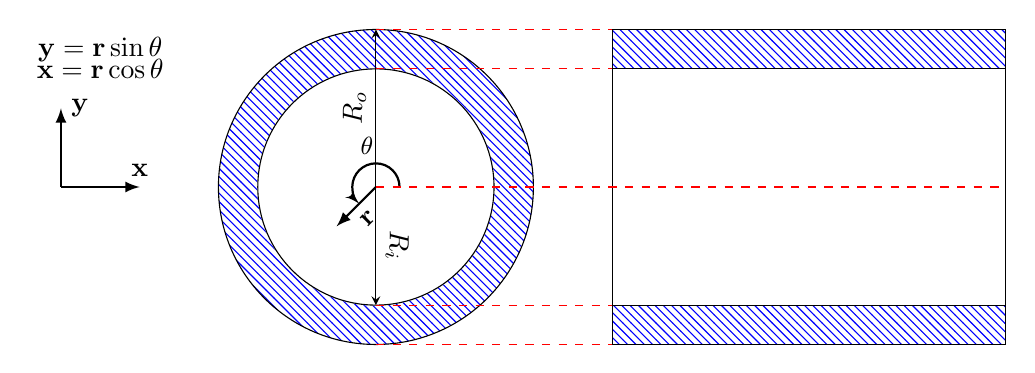
\begin{tikzpicture}
\draw [fill,black,pattern=north west lines, pattern color=blue](0,0) circle(2);
\draw [fill,white](0,0) circle(1.5);\draw [black](0,0) circle(1.5);
\draw [->,>=stealth] (0,0)--(0,-1.5) node[midway,above,sloped]{$R_i$};
\draw [->,>=stealth] (0,0)--(0,2)node[midway,above,sloped]{$R_o$};
\draw [->,>=latex,thick] (0,0)--(-0.5,-0.5)node[midway,below,sloped]{$\mathbf{r}$};
\draw[->,>=latex',thick] (0.3,0) arc[radius=0.3, start angle=0, end angle=225] node[midway,above] {\small$\mathbf{\theta}$};
\draw [fill,black,pattern=north west lines, pattern color=blue](3,-2) rectangle (8,2);
\draw [black,fill,white](3,-1.5) rectangle (8,1.5);
\draw [black](3,-1.5) rectangle (8,1.5);

\draw [dashed,red] (0,0)--(8,0);
\draw [dashed,red] (0,2)--(3,2);
\draw [dashed,red] (0,-2)--(3,-2);
\draw [dashed,red] (0,-1.5)--(3,-1.5);
\draw [dashed,red] (0,1.5)--(3,1.5);

\draw [thick,->,>=latex] (-4,0) -- (-3,0) node[above]{$\mathbf{x}$};
\draw [thick,->,>=latex] (-4,0) -- (-4,1) node[right]{$\mathbf{y}$};
\draw [](-3.5,1.5) node[]{$\mathbf{x}=\mathbf{r}\cos\mathbf{\theta}$};
\draw [](-3.5,1.75) node[]{$\mathbf{y}=\mathbf{r}\sin\mathbf{\theta}$};

\end{tikzpicture}
\caption{هندسه مسئله لامه.}\label{fig01geom}
\end{figure}
$C_1$ و $C_2$ ثابت‌هایی است که با اعمال شرایط مرزی مشخص می‌گردد.
\begin{equation}\nonumber
\begin{aligned}
\sigma_r(r=R_i) = &-P_i= \frac{E}{1-\nu^2}\left[C_1(1+\nu)-C_2(1-\nu)\frac{1}{R_i^2}\right]\\
\sigma_r(r=R_o) = &-P_o=0=\frac{E}{1-\nu^2}\left[C_1(1+\nu)-C_2(1-\nu)\frac{1}{R_o^2}\right]\\
\end{aligned}
\end{equation}
با حل این معادلات،
\begin{equation}\nonumber
\begin{aligned}
C_1=&\frac{1-\nu}{E}\frac{P_iR_i^2-P_oR_o^2}{R_o^2-R_i^2}\\
C_2=&\frac{1+\nu}{E}\frac{R_i^2-R_o^2}{R_o^2-R_i^2}\left(P_i-P_o\right)
\end{aligned}
\end{equation}
با جایگذاری این مقادیر داریم،
\begin{equation}\label{eqs04}
\begin{aligned}
\sigma_{r}=&\frac{P_i R_i^{2}-P_o R_o^{2}}{R_o^{2}-R_i^{2}}-\frac{R_i^{2} R_o^{2}}{r^{2}} \frac{P_i-P_o}{R_o^{2}-R_i^{2}}\\
\sigma_{\theta}=&\frac{P_i R_i^{2}-P_o R_o^{2}}{R_o^{2}-R_i^{2}}+\frac{R_i^{2} R_o^{2}}{r^{2}} \frac{P_i-P_o}{R_o^{2}-R_i^{2}}
\end{aligned}
\end{equation}
\subsubsection{تنش مسطح با تنها فشار داخلی}
اگر فشار خارجی 
$P_o=0$
باشد،
%\begin{equation}\nonumber
\begin{align}
\sigma_{r}=&\frac{P_i R_i^{2}}{R_o^{2}-R_i^{2}}\left[1-\frac{R_o^2}{r^2}\right]\label{eqs01}\\
\sigma_{\theta}=&\frac{P_i R_i^{2}}{R_o^{2}-R_i^{2}}\left[1+\frac{R_o^2}{r^2}\right]\label{eqs02}\\
\end{align}
%\end{equation}
این روابط نشان می‌دهد که $\sigma_r$ کماکان تنشی فشاری یا منفی و $\sigma_\theta$ تنشی کششی یا مثبت است.
\begin{figure}\centering
\begin{subfigure}{0.45\textwidth}
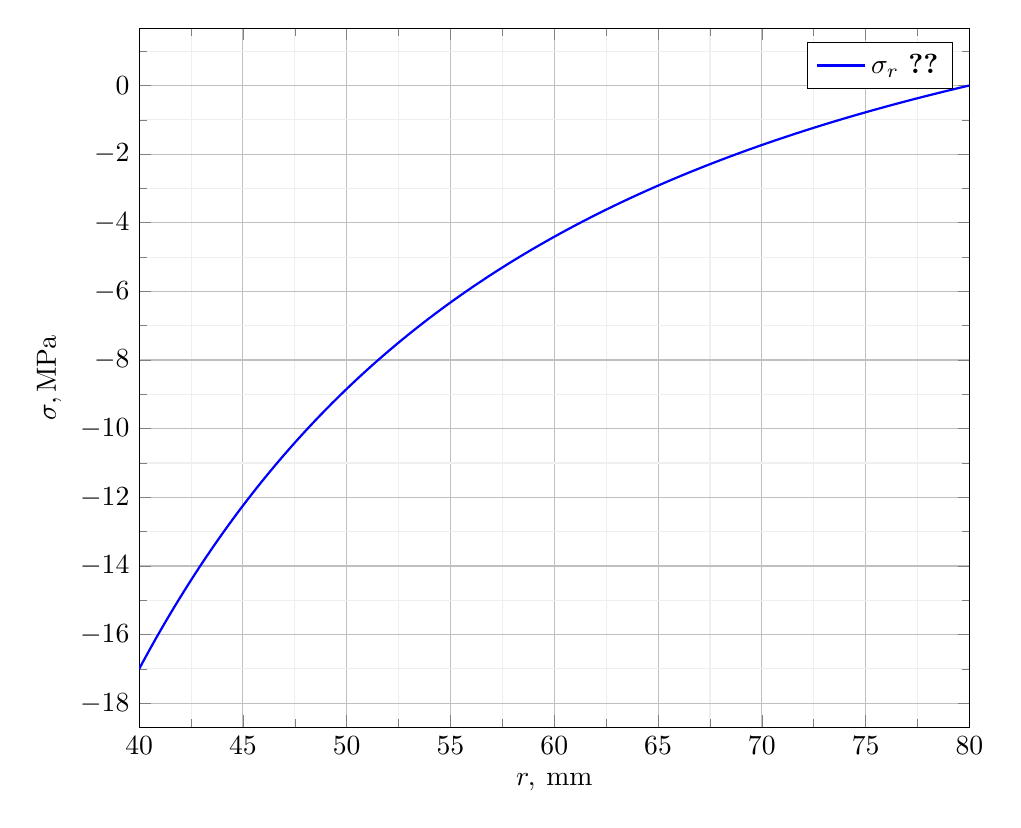
\begin{tikzpicture}
\begin{axis}[
	xmin = 40, xmax = 80,
%	xtick distance = 2.5,
%	ytick distance = 0.5,
	grid = both,
	minor tick num = 1,
	major grid style = {lightgray},
	minor grid style = {lightgray!25},
	width = \textwidth,
	ylabel = {$\sigma,\mathrm{MPa}$},
	xlabel = {$r,\:\mathrm{mm}$},
%	height = 0.5\textwidth,
]
	\addplot[
		domain = 40:80,
		samples = 200,
		smooth,
		thick,
		blue,
	] {17*40^2/(80^2-40^2)*(1-80^2/x^2)};
	\addlegendentry{\rl{$\sigma_r$ \cref{eqs01}}}
\end{axis}
\end{tikzpicture}\end{subfigure}\:\:\:\:\:\:\:\:\begin{subfigure}{0.45\textwidth}
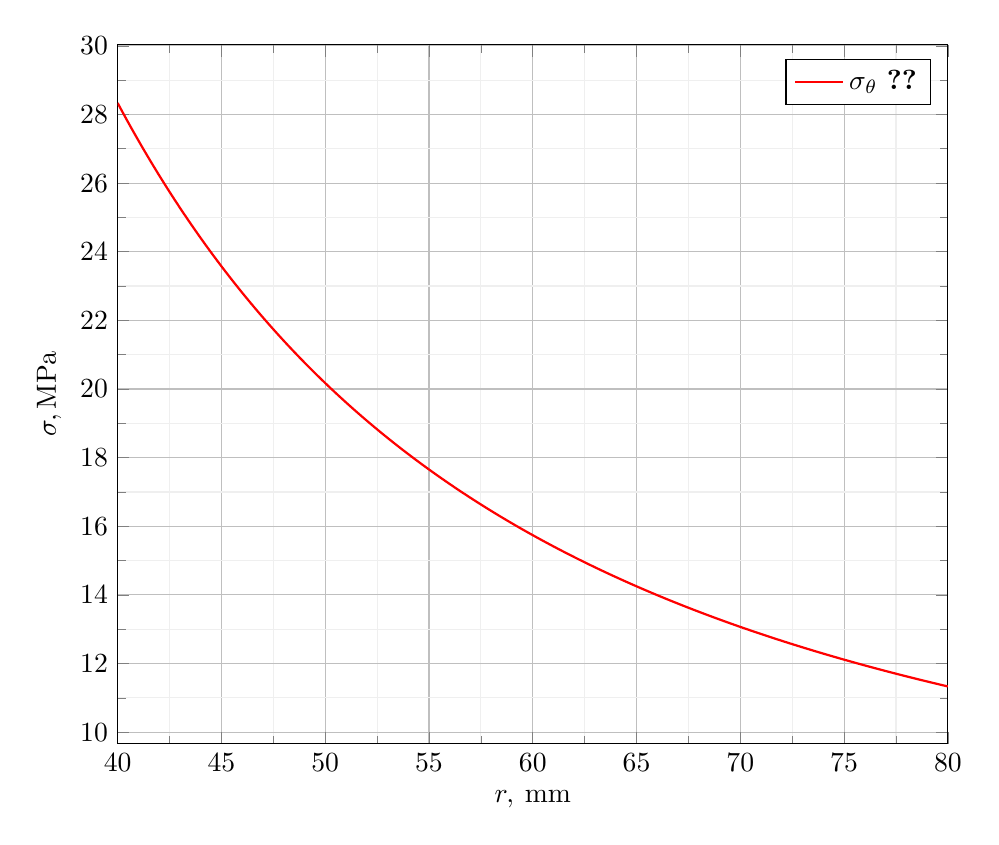
\begin{tikzpicture}
\begin{axis}[
	xmin = 40, xmax = 80,
%	xtick distance = 2.5,
%	ytick distance = 0.5,
	grid = both,
	minor tick num = 1,
	major grid style = {lightgray},
	minor grid style = {lightgray!25},
	width = \textwidth,
	ylabel = {$\sigma,\mathrm{MPa}$},
	xlabel = {$r,\:\mathrm{mm}$},
%	height = 0.5\textwidth,
]
	\addplot[
		domain = 40:80,
		samples = 200,
		smooth,
		thick,
		red,
	]{17*40^2/(80^2-40^2)*(1+80^2/x^2)};
	\addlegendentry{\rl{$\sigma_\theta$ \cref{eqs02}}}
\end{axis}
\end{tikzpicture}\end{subfigure}
\end{figure}
\subsection{کرنش مسطح}
به همین ترتیب برای کنش مسطح، فرض بر تغییر نکردن $\sigma_z$ در راستای محور $z$ است، مطابق \cref{eq1}
\begin{equation}\nonumber
\frac{\mathrm{d}}{\mathrm{d}r}(r\sigma_r)-\sigma_\theta=0
\end{equation}
از قانون هوک\cite{hooke1678}،


\begin{equation}\nonumber
\begin{aligned}
\varepsilon_{r}=&\frac{1}{E}\left[\sigma_{r}-v\left(\sigma_{\theta}+\sigma_{z}\right)\right]\\
\varepsilon_{\theta}=&\frac{1}{E}\left[\sigma_{\theta}-v\left(\sigma_{r}+\sigma_{z}\right)\right]\\
\varepsilon_{z}=&\frac{1}{E}\left[\sigma_{r}-v\left(\sigma_{r}+\sigma_{\theta}\right)\right]
\end{aligned}
\end{equation}
با
 $\varepsilon_z=0$
\begin{equation}\nonumber
\begin{aligned}
\sigma_{z}=&v\left(\sigma_{r}+\sigma_{\theta}\right)\\
\varepsilon_{r}=&\frac{1+v}{E}\left[(1-v) \sigma_{r}-v \sigma_{\theta}\right]\\
\varepsilon_{\theta}=&\frac{1+v}{E}\left[(1-v) \sigma_{\theta}-v \sigma_{r}\right]
\end{aligned}
\end{equation}
با حل برای تنش،

\begin{equation}\nonumber
\begin{aligned}
\sigma_{\theta}=&\frac{E}{(1-2 v)(1+v)}\left[v \varepsilon_{r}+(1-v) \varepsilon_{\theta}\right]\\
\sigma_{r}=&\frac{E}{(1-2 v)(1+v)}\left[(1-v) \varepsilon_{r}+v \varepsilon_{\theta}\right]
\end{aligned}\end{equation}
و با جایگذاری کرنش،
\begin{equation}\label{eq4}
\begin{aligned}
\sigma_{r}=&\frac{E}{(1-2 v)(1+v)}\left[(1-v) \frac{d u_{r}}{d r}+v \frac{u_{r}}{r}\right]\\
\sigma_{\theta}=&\frac{E}{(1-2 v)(1+v)}\left[v \frac{d u_{r}}{d r}+(1-v) \frac{u_{r}}{r}\right]\\
\end{aligned}
\end{equation}
با جایگذاری این روابط در معادلات تعادل،
\begin{equation}\nonumber\begin{aligned}
\frac{\mathrm{d}}{\mathrm{d} r}\left[(1-v) r \frac{d u_{r}}{d r}+v u_{r}\right]-v \frac{d u_{r}}{d r}-(1-v) \frac{u_{r}}{r}&=0\\
\frac{d u_{r}}{d r}+r \frac{\mathrm{d}^{2} u_{r}}{\mathrm{d} r^{2}}-\frac{u_{r}}{r}&=0\\
\frac{\mathrm{d}}{\mathrm{d} r}\left(\frac{\mathrm{d} u}{\mathrm{d} r}+\frac{u_{r}}{r}\right)&=0
\end{aligned}
\end{equation}
با فرض \cref{eqs03} برای $u_r$ و جایگذاری در \cref{eq4} داریم
\begin{equation}\nonumber\begin{aligned}
\sigma_{\theta}=&\frac{E}{(1-2 v)(1+v)}\left[C_{1}+(1-2 v) \frac{C_{2}}{r^{2}}\right]\\
\sigma_{r}=&\frac{E}{(1-2 v)(1+v)}\left[C_{1}-(1-2 v) \frac{C_{2}}{r^{2}}\right]
\end{aligned}
\end{equation}
بر اساس حدود مرزی،
\begin{equation}\nonumber
\begin{aligned}
\sigma_r(r=R_i)=&-P_i=\frac{E}{(1-2 v)(1+v)}\left[C_{1}-(1-2 v) \frac{C_{2}}{R_i^{2}}\right]\\
\sigma_r(r=R_o)=&-P_{o}=\frac{E}{(1-2 v)(1+v)}\left[C_{1}+(1-2 v) \frac{C_{2}}{R_o^{2}}\right]
\end{aligned}
\end{equation}
درنتیجه،
\begin{equation}\nonumber\begin{aligned}
C_{1}=&\frac{(1-2 v)(1+v)}{E} \frac{P_{o} R_o^{2}-P_{i} R_i^{2}}{R_i^{2}-R_o^{2}}\\
C_{2}=&\frac{1+v}{E} \frac{\left(P_{o}-P_{i}\right) R_i^{2} R_o^{2}}{R_i^{2}-R_o^{2}}
\end{aligned}
\end{equation}
با جایگذاری این روابط داریم،
\begin{equation}\nonumber\begin{aligned}
\sigma_{r}=&\frac{P_{i} R_i^{2}-P_{o} R_o^{2}}{R_o^{2}-R_i^{2}}-\frac{R_i^{2} R_o^{2}}{r^{2}} \frac{P_{i}-P_{o}}{R_o^{2}-R_i^{2}} \\
\sigma_{\theta}=&\frac{P_{i} R_i^{2}-P_{o} R_o^{2}}{R_o^{2}-R_i^{2}}+\frac{R_i^{2} R_o^{2}}{r^{2}} \frac{P_{i}-P_{o}}{R_o^{2}-R_i^{2}}
\end{aligned}
\end{equation}
که معادل \cref{eqs04} است.
\section{مدلسازی در \lr{MATLAB}}\label{sec_numm}
یک استوانه با شعاع داخلی 
$R_i=40\mathrm{mm}$
 و شعاع خارجی 
 $R_o=80\mathrm{mm}$
  و به طول 
  $L=1000\mathrm{mm}$
   تحت فشار داخلی 
   $17\mathrm{MPa}$
    با استفاده از جعبه ابزار مکانیک سازه \lr{MATLAB} مدلسازی شد. از المان‌های شش وجهی درجه 
    $2$
     برای مش استفاده گردید. کمینه اندازه المان 
     $1\mathrm{mm}$
      و بیشینه آن 
      $10\mathrm{mm}$
       است.

\begin{figure}\centering
\includegraphics[width=0.4\textwidth]{Figures/fig01.pdf}
\caption{هندسه مدل سه بعدی.}\label{fig01}
\end{figure}
\begin{figure}\centering
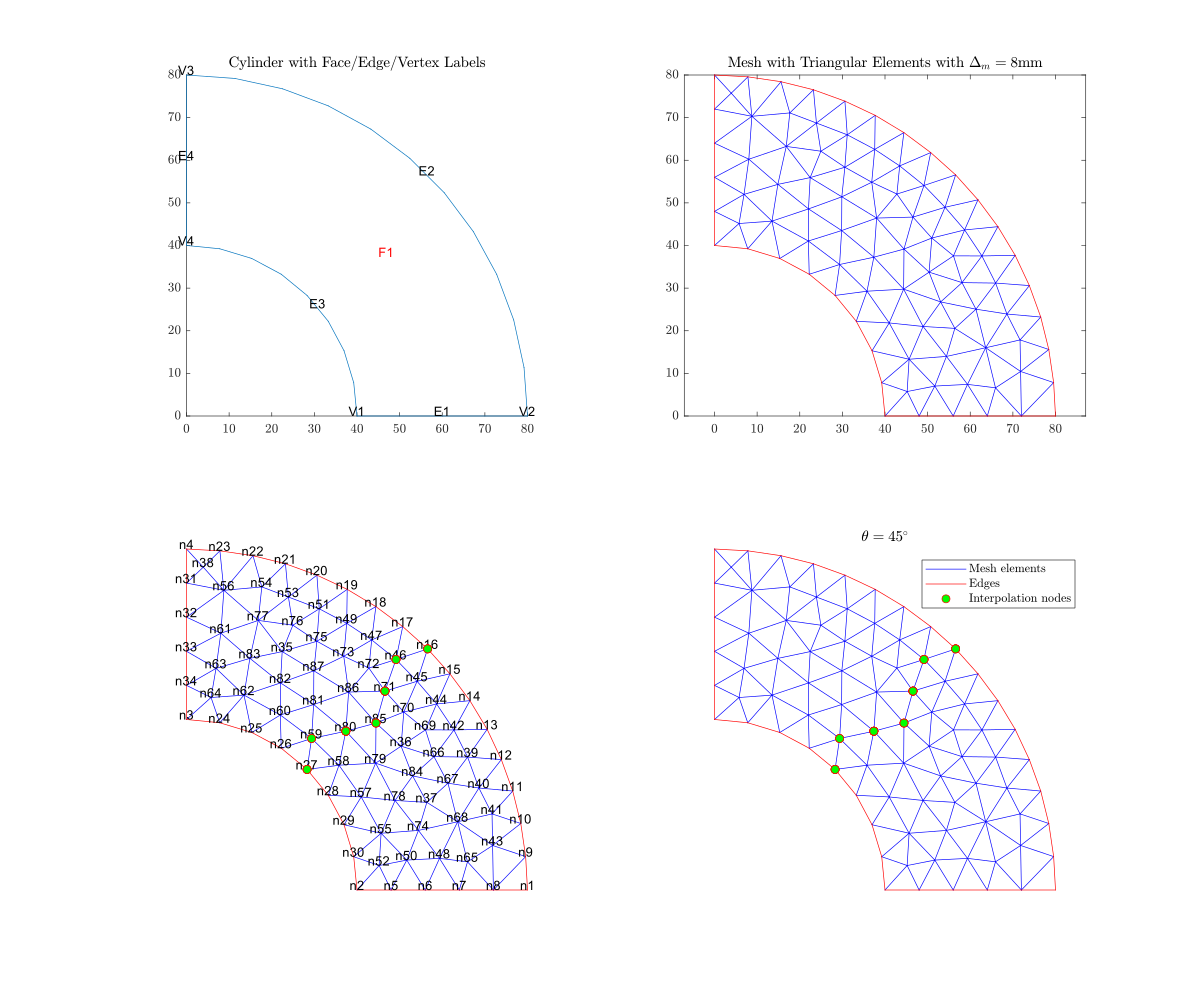
\includegraphics[width=\textwidth, trim={3cm 3cm 1cm 1cm},clip]{Figures/fig01m8.pdf}
\caption{مش و مدل دو بعدی.}\label{fig01m}
\end{figure}
\begin{figure}\centering
\begin{subfigure}{\textwidth}\centering
\includegraphics[width=0.8\textwidth,trim={1cm 1cm 1cm 0cm},clip]{Figures/fig03m8.pdf}
\caption{خروجی مدل \lr{2D}.}\label{fig05a}
\end{subfigure}
\begin{subfigure}{\textwidth}\centering
%\input{Figures/fig05}
\includegraphics[width=0.8\textwidth,trim={1cm 1cm 1cm 0cm},clip]{Figures/fig05m10.pdf}
\caption{خروجی مدل \lr{3D}.}\label{fig05b}
\end{subfigure}
\caption{تغییرات تنش در شعاع.}\label{fig05}
\end{figure}

\begin{figure}\centering
%\input{Figures/fig06}
\includegraphics[width=0.8\textwidth,trim={1cm 1cm 1cm 0cm},clip]{Figures/fig06m10.pdf}
\caption{تغییرات تنش در طول.}\label{fig06}
\end{figure}
\section{نتایج}
\begin{itemize} 
\item مدل عددی متناسب \pcref{sec_numm} با روابط نظری \pcref{sec_theory} اثبات شده است\pcref{fig05}.
\item مدل عددی \pcref{sec_numm} و اثبات ریاضی \pcref{sec_theory} جفت نشان دهنده افت جفت تنش شعاعی $\sigma_r$ و زاویه‌ای $\sigma_\theta$ با افزایش شعاع $r$ است\pcref{fig05}.
\item همچنین تنش در راستای طولی مطابق خروجی عددی ثابت می‌ماند که بیان کننده برقراری فرض تنش یا کرنش مسطح است\pcref{fig06}. 
\item نوسان تنش در انتهای بازه نمودار \cref{fig06} نشان دهنده حساسیت شدید مدل به شرایط مرزی و اندازه مش است. این نوسانات با افزایش اندازه مش کاسته می‌شود.
\end{itemize}
\newpage
\section{پیوست}\subsection{تبدیل تنش از مختصات کارتزی به استوانه‌ای}
\includepdf[pages=-]{main.pdf}
%از \url{http://solidmechanics.org/text/AppendixD/AppendixD.htm} داریم:
%\begin{equation}
%\left[\begin{array}{ccc}
%S_{r r} & S_{r \theta} & S_{r z} \\
%S_{\theta r} & S_{\theta \theta} & S_{\theta z} \\
%S_{z r} & S_{\theta z} & S_{z z}
%\end{array}\right]=\left[\begin{array}{ccc}
%\cos \theta & \sin \theta & 0 \\
%-\sin \theta & \cos \theta & 0 \\
%0 & 0 & 1
%\end{array}\right]\left[\begin{array}{lll}
%S_{x x} & S_{x y} & S_{x z} \\
%S_{y x} & S_{\theta \theta} & S_{\theta z} \\
%S_{z r} & S_{\theta z} & S_{z z}
%\end{array}\right]\left[\begin{array}{ccc}
%\cos \theta & -\sin \theta & 0 \\
%\sin \theta & \cos \theta & 0 \\
%0 & 0 & 1
%\end{array}\right]
%\end{equation}
%دو ماتریس اول را در هم ضرب می‌کنیم:
%
%برای سهولت قیدهای فضایی، تبدیل‌های زیر تعریف شده است:
%\begin{equation}
%\begin{aligned}
%&\begin{aligned}
%\cos \theta & =\mathbf{c}_\theta \\
%\sin \theta & =\mathbf{s}_\theta
%\end{aligned}\\
%&\begin{aligned}
%& {\left[\begin{array}{ccc}
%\cos \theta & \sin \theta & 0 \\
%-\sin \theta & \cos \theta & 0 \\
%0 & 0 & 1
%\end{array}\right] } {\left[\begin{array}{ccc}
%S_{x x} & S_{x y} & S_{x z} \\
%S_{y x} & S_{\theta \theta} & S_{\theta z} \\
%S_{z r} & S_{\theta z} & S_{z z}
%\end{array}\right] } \\
%& \Longrightarrow\left[\begin{array}{ccc}
%\mathbf{c}_\theta S_{x x}+\mathbf{s}_\theta S_{y x}+0 & \mathbf{c}_\theta S_{x y}+\mathbf{s}_\theta S_{y y}+0 & \mathbf{c}_\theta S_{x z}+\mathbf{s}_\theta S_{y z}+0 \\
%-\mathbf{s}_\theta S_{x x}+\mathbf{c}_\theta S_{y x}+0 & -\mathbf{s}_\theta S_{x y}+\mathbf{c}_\theta S_{y y}+0 & -\mathbf{s}_\theta S_{x z}+\mathbf{c}_\theta S_{y z}+0 \\
%0+0+S_{z x} & 0+0+S_{z y} & 0+0+S_{z z}
%\end{array}\right] \\
%& 0+\left[\begin{array}{ccc}
%\mathbf{c}_\theta S_{x x}+\mathbf{s}_\theta S_{y x} & \mathbf{c}_\theta S_{x y}+\mathbf{s}_\theta S_{y y} & \mathbf{c}_\theta S_{x z}+\mathbf{s}_\theta S_{y z} \\
%-\mathbf{s}_\theta S_{x x}+\mathbf{c}_\theta S_{y x} & -\mathbf{s}_\theta S_{x y}+\mathbf{c}_\theta S_{y y} & -\mathbf{s}_\theta S_{x z}+\mathbf{c}_\theta S_{y z} \\
%S_{z x} & S_{z y} & S_{z z}
%\end{array}\right]
%\end{aligned}
%\end{aligned}
%\end{equation}
%نتیجه را در ماتریس سوم ضرب می‌کنیم:
%\begin{equation}
%\begin{aligned}
%& {\left[\begin{array}{ccc}
%\mathbf{c}_\theta S_{x x}+\mathbf{s}_\theta S_{y x} & \mathbf{c}_\theta S_{x y}+\mathbf{s}_\theta S_{y y} & \mathbf{c}_\theta S_{x z}+\mathbf{s}_\theta S_{y z} \\
%-\mathbf{s}_\theta S_{x x}+\mathbf{c}_\theta S_{y x} & -\mathbf{s}_\theta S_{x y}+\mathbf{c}_\theta S_{y y} & -\mathbf{s}_\theta S_{x z}+\mathbf{c}_\theta S_{y z} \\
%S_{z x} & S_{z y} & S_{z z}
%\end{array}\right]\left[\begin{array}{ccc}
%\cos \theta & -\sin \theta & 0 \\
%\sin \theta & \cos \theta & 0 \\
%0 & 0 & 1
%\end{array}\right]=} \\
%& {\left[\begin{array}{ccc}
%\mathbf{c}_\theta^2 S_{x x}+\mathbf{s}_\theta \mathbf{c}_\theta S_{y x}+\mathbf{c}_\theta \mathbf{s}_\theta S_{x y}+\mathbf{s}_\theta^2 S_{y y} & -\mathbf{c}_\theta \mathbf{s}_\theta S_{x x}-\mathbf{s}_\theta^2 S_{y x}+\mathbf{c}_\theta^2 S_{x y}+\mathbf{c}_\theta \mathbf{s}_\theta S_{y y} & \mathbf{c}_\theta S_{x y}+\mathbf{s}_\theta S_{y z} \\
%-\mathbf{s}_\theta \mathbf{c}_\theta S_{x x}+\mathbf{c}_\theta^2 S_{y x}-\mathbf{s}_\theta^2 S_{x y}+\mathbf{c}_\theta \mathbf{s}_\theta S_{y y} & \mathbf{s}_\theta^2 S_{x x}-\mathbf{c}_\theta \mathbf{s}_\theta S_{y x}-\mathbf{c}_\theta \mathbf{s}_\theta S_{x y}+\mathbf{c}_\theta^2 S_{y y} & -\mathbf{s}_\theta S_{x z}+\mathbf{c}_\theta S_{y z} \\
%\mathbf{c}_\theta S_{z x}+\mathbf{s}_\theta S_{z y} & -\mathbf{s}_\theta S_{z x}+\mathbf{c}_\theta S_{z y} & S_{z z}
%\end{array}\right]} \\
%&
%\end{aligned}
%\end{equation}
%با فرض متقارن بودن تانسور ($S_{ij}=S_{ji}$):
%\begin{equation}
%(5) \Longrightarrow\left[\begin{array}{ccc}
%\mathbf{c}_\theta^2 S_{x x}+2 \mathbf{c}_\theta \mathbf{s}_\theta S_{x y}+\mathbf{s}_\theta^2 S_{y y} & -\mathbf{c}_\theta \mathbf{s}_\theta S_{x x}+\left(\mathbf{c}_\theta^2-\mathbf{s}_\theta^2\right) S_{x y}+\mathbf{c}_\theta \mathbf{s}_\theta S_{y y} & \mathbf{c}_\theta S_{x z}+\mathbf{s}_\theta S_{y z} \\
%-\mathbf{c}_\theta \mathbf{s}_\theta S_{x x}+\left(\mathbf{c}_\theta^2-\mathbf{s}_\theta^2\right) S_{x y}+\mathbf{c}_\theta \mathbf{s}_\theta S_{y y} & \mathbf{s}_\theta S_{x x}-2 \mathbf{c}_\theta \mathbf{s}_\theta S_{x y}+\mathbf{c}_\theta^2 S_{y y} & -\mathbf{s}_\theta S_{x z}+\mathbf{c}_\theta S_{y z} \\
%\mathbf{c}_\theta S_{x z}+\mathbf{s}_\theta S_{y z} & -\mathbf{s}_\theta S_{x z}+\mathbf{c}_\theta S_{y z} & S_{z z}
%\end{array}\right]
%\end{equation}
%
%\begin{equation}
%\left[\begin{array}{lll}
%S_{r r} & S_{r \theta} & S_{r z} \\
%S_{\theta r} & S_{\theta \theta} & S_{\theta z} \\
%S_{z r} & S_{\theta z} & S_{z z}
%\end{array}\right]=\left[\begin{array}{ccc}
%\mathbf{c}_\theta^2 S_{x x}+2 \mathbf{c}_\theta \mathbf{s}_\theta S_{x y}+\mathbf{s}_\theta^2 S_{y y} & \mathbf{c}_\theta \mathbf{s}_\theta\left(S_{y y}-S_{x x}\right)+\left(\mathbf{c}_\theta^2-\mathbf{s}_\theta^2\right) S_{x y} & \mathbf{c}_\theta S_{x z}+\mathbf{s}_\theta S_{y z} \\
%\mathbf{c}_\theta \mathbf{s}_\theta\left(S_{y y}-S_{x x}\right)+\left(\mathbf{c}_\theta^2-\mathbf{s}_\theta^2\right) S_{x y} & \mathbf{s}_\theta^2 S_{x x}-2 \mathbf{c}_\theta \mathbf{s}_\theta S_{x y}+\mathbf{c}_\theta^2 S_{y y} & -\mathbf{s}_\theta S_{x z}+\mathbf{c}_\theta S_{y z} \\
%\mathbf{c}_\theta S_{x z}+\mathbf{s}_\theta S_{y z} & -\mathbf{s}_\theta S_{x z}+\mathbf{c}_\theta S_{y z} & S_{z z}
%\end{array}\right]
%\end{equation}
%
%داریم:
%
%\begin{equation}
%\begin{aligned}
%& S_{r r}=\mathbf{c}_\theta^2 S_{x x}+2 \mathbf{c}_\theta \mathbf{s}_\theta S_{x y}+\mathbf{s}_\theta^2 S_{y y} \\
%& S_{r \theta}=\mathbf{c}_\theta \mathbf{s}_\theta\left(S_{y y}-S_{x x}\right)+\left(\mathbf{c}_\theta^2-\mathbf{s}_\theta^2\right) S_{x y} \\
%& S_{r z}=\mathbf{c}_\theta S_{x z}+\mathbf{s}_\theta S_{y z} \\
%& S_{\theta \theta}=\mathbf{s}_\theta^2 S_{x x}-2 \mathbf{c}_\theta \mathbf{s}_\theta S_{x y}+\mathbf{c}_\theta^2 S_{y y} \\
%& S_{\theta z}=-\mathbf{s}_\theta S_{x z}+\mathbf{c}_\theta S_{y z} \\
%& S_{z z}=S_{z z}
%\end{aligned}
%\end{equation}
\subsection{کد مدل \lr{3D}}
\begin{latin}
\lstinputlisting[style=Matlab-editor]{listing_publish.m}
\end{latin}
\subsection{کد مدل \lr{2D}}
\begin{latin}
\lstinputlisting[style=Matlab-editor]{develop_2d.m}
\end{latin}
\subsection{پایتون تولید هندسه در \lr{ABAQUS}}

\begin{latin}
\inputpython{mesh2d.jnl}{1}{69}
%\lstinputlisting[style=Matlab-Pyglike]{mesh2d.jnl}
\end{latin}

\bibliographystyle{unsrt-fa}
\bibliography{main_bibs}
\end{document}